%%%%%%%%%%%%%%%%%%%%%%%%%%%%%%%%%%%%%%%%%%%%%%%
%
% Template per Elaborato di Laurea
% DISI - Dipartimento di Ingegneria e Scienza dell’Informazione
%
% update 2015-09-10
%
% Per la generazione corretta del 
% pdflatex nome_file.tex
% bibtex nome_file.aux
% pdflatex nome_file.tex
% pdflatex nome_file.tex
%
%%%%%%%%%%%%%%%%%%%%%%%%%%%%%%%%%%%%%%%%%%%%%%%

% formato FRONTE RETRO
\documentclass[a4paper,11pt,titlepage,twoside,openany]{book}
\usepackage{epsfig}
\usepackage{plain}
\usepackage{setspace}
\usepackage[paperheight=29.7cm,paperwidth=21cm,outer=1.5cm,inner=2.5cm,top=2cm,bottom=2cm]{geometry} % per definizione layout
\usepackage{titlesec} % per formato custom dei titoli dei capitoli
\usepackage{fancyvrb} % per verbatim numerato

%%%%%%%%%%%%%%
% supporto lettere accentate
%
%\usepackage[latin1]{inputenc} % per Windows;
\usepackage[utf8x]{inputenc} % per Linux (richiede il pacchetto unicode);
%\usepackage[applemac]{inputenc} % per Mac.

\singlespacing

\usepackage[italian]{babel}

\begin{document}

  % nessuna numerazione
  \pagenumbering{gobble} 
  \pagestyle{plain}

\thispagestyle{empty}

\begin{center}
  \begin{figure}[h!]
    \centerline{
\psfig{file=marchio_unitrento_colore_it_202002.eps,width=0.6\textwidth}}
  \end{figure}

  \vspace{2 cm} 

  \LARGE{Dipartimento di Ingegneria e Scienza dell’Informazione\\}

  \vspace{1 cm} 
  \Large{Corso di Laurea in\\
    Ingegneria Informatica, delle Comunicazioni ed Elettronica
    %Informatica
    %Ingegneria dell'Informazione e delle Comunicazioni
    %Ingegneria dell'Informazione e Organizzazione d'Impresa
    %Ingegneria Elettronica e delle Telecomunicazioni
  }

  \vspace{2 cm} 
  \Large\textsc{Elaborato finale\\} 
  \vspace{1 cm} 
  \Huge\textsc{Prolog planner\\}
  \Large{\it{Task planner logico per la manipolazioni di blocchi tramite un UR5}}


  \vspace{2 cm} 
  \begin{tabular*}{\textwidth}{ c @{\extracolsep{\fill}} c }
  \Large{Supervisore} & \Large{Laureando}\\
  \Large{Prof. Luigi Palopoli}& \Large{Davide De Martini}\\
  \end{tabular*}

  \vspace{2 cm} 

  \Large{Anno accademico 2022/2023}
  
\end{center}



  \clearpage
 
%%%%%%%%%%%%%%%%%%%%%%%%%%%%%%%%%%%%%%%%%%%%%%%%%%%%%%%%%%%%%%%%%%%%%%%%%%
%%%%%%%%%%%%%%%%%%%%%%%%%%%%%%%%%%%%%%%%%%%%%%%%%%%%%%%%%%%%%%%%%%%%%%%%%%
%% Nota
%%%%%%%%%%%%%%%%%%%%%%%%%%%%%%%%%%%%%%%%%%%%%%%%%%%%%%%%%%%%%%%%%%%%%%%%%%
%% Sezione Ringraziamenti opzionale
%%%%%%%%%%%%%%%%%%%%%%%%%%%%%%%%%%%%%%%%%%%%%%%%%%%%%%%%%%%%%%%%%%%%%%%%%%
%%%%%%%%%%%%%%%%%%%%%%%%%%%%%%%%%%%%%%%%%%%%%%%%%%%%%%%%%%%%%%%%%%%%%%%%%%
  \thispagestyle{empty}

\begin{center}
  {\bf \Huge Ringraziamenti}
\end{center}

\vspace{4cm}


\emph{
  A tutti
}

  \clearpage
  \pagestyle{plain} % nessuna intestazione e pie pagina con numero al centro

  
  % inizio numerazione pagine in numeri arabi
  \mainmatter

%%%%%%%%%%%%%%%%%%%%%%%%%%%%%%%%%%%%%%%%%%%%%%%%%%%%%%%%%%%%%%%%%%%%%%%%%%
%%%%%%%%%%%%%%%%%%%%%%%%%%%%%%%%%%%%%%%%%%%%%%%%%%%%%%%%%%%%%%%%%%%%%%%%%%
%% Nota
%%%%%%%%%%%%%%%%%%%%%%%%%%%%%%%%%%%%%%%%%%%%%%%%%%%%%%%%%%%%%%%%%%%%%%%%%%
%% Si ricorda che il numero massimo di facciate e' 30.
%% Nel conteggio delle facciate sono incluse 
%%   indice
%%   sommario
%%   capitoli
%% Dal conteggio delle facciate sono escluse
%%   frontespizio
%%   ringraziamenti
%%   allegati    
%%%%%%%%%%%%%%%%%%%%%%%%%%%%%%%%%%%%%%%%%%%%%%%%%%%%%%%%%%%%%%%%%%%%%%%%%%
%%%%%%%%%%%%%%%%%%%%%%%%%%%%%%%%%%%%%%%%%%%%%%%%%%%%%%%%%%%%%%%%%%%%%%%%%%

    % indice
    \tableofcontents
    \clearpage
    
    
          
    % gruppo per definizone di successione capitoli senza interruzione di pagina
    \begingroup
      % nessuna interruzione di pagina tra capitoli
      % ridefinizione dei comandi di clear page
      \renewcommand{\cleardoublepage}{} 
      \renewcommand{\clearpage}{} 
      % redefinizione del formato del titolo del capitolo
      % da formato
      %   Capitolo X
      %   Titolo capitolo
      % a formato
      %   X   Titolo capitolo
      
      \titleformat{\chapter}
        {\normalfont\Huge\bfseries}{\thechapter}{1em}{}
        
      \titlespacing*{\chapter}{0pt}{0.59in}{0.02in}
      \titlespacing*{\section}{0pt}{0.20in}{0.02in}
      \titlespacing*{\subsection}{0pt}{0.10in}{0.02in}
      
      % sommario
      \chapter*{Sommario} % senza numerazione
\label{sommario}

\addcontentsline{toc}{chapter}{Sommario} % da aggiungere comunque all'indice
  Sommario è un breve riassunto del lavoro svolto dove si descrive l'obiettivo, l'oggetto della tesi, le 
metodologie e le tecniche usate, i dati elaborati e la spiegazione delle conclusioni alle quali siete arrivati.  

Il sommario dell’elaborato consiste al massimo di 3 pagine e deve contenere le seguenti informazioni:
\begin{itemize}
  \item contesto e motivazioni 
  \item breve riassunto del problema affrontato
  \item tecniche utilizzate e/o sviluppate
  \item risultati raggiunti, sottolineando il contributo personale del laureando/a
\end{itemize}





%%%%%%%%%%%%%%%%%%%%%%%%%%%%%%%%%%%%%%%%%%%%%%%%%%%%%%%%%%%%%%%%%%%%%%%%%%
%%%%%%%%%%%%%%%%%%%%%%%%%%%%%%%%%%%%%%%%%%%%%%%%%%%%%%%%%%%%%%%%%%%%%%%%%%
%% Nota
%%%%%%%%%%%%%%%%%%%%%%%%%%%%%%%%%%%%%%%%%%%%%%%%%%%%%%%%%%%%%%%%%%%%%%%%%%
%% Sommario e' un breve riassunto del lavoro svolto dove si descrive 
%% l’obiettivo, l’oggetto della tesi, le metodologie e 
%% le tecniche usate, i dati elaborati e la spiegazione delle conclusioni 
%% alle quali siete arrivati.
%% Il sommario dell’elaborato consiste al massimo di 3 pagine e deve contenere le seguenti informazioni: 
%%   contesto e motivazioni
%%   breve riassunto del problema affrontato
%%   tecniche utilizzate e/o sviluppate
%%   risultati raggiunti, sottolineando il contributo personale del laureando/a
%%%%%%%%%%%%%%%%%%%%%%%%%%%%%%%%%%%%%%%%%%%%%%%%%%%%%%%%%%%%%%%%%%%%%%%%%%
%%%%%%%%%%%%%%%%%%%%%%%%%%%%%%%%%%%%%%%%%%%%%%%%%%%%%%%%%%%%%%%%%%%%%%%%%%      
      
      %%%%%%%%%%%%%%%%%%%%%%%%%%%%%%%%
      % lista dei capitoli
      %
      % \input oppure \include
      %
      \clearpage
\newpage
\chapter{Introduzione}
\label{cha:intro}

% - INTRODUZIONE AL TEMA
% - MOTIVI DEL CASO DI STUDIO
% - OBIETTIVI DEL LAVORO
% - STRUTTURA 

In questo primo capitolo viene introdotto il caso di studio, partendo dalla definizione del problema, descrivendo poi gli obiettivi desiderati
e concludendo con una spiegazione della struttura della tesi.

% INTRODUZIONE AL TEMA
Per la mia tesi triennale mi sono voluto concentrare sul campo dell'intelligenza artificiale e la robotica. Il caso di studio identificato
dal prof. Luigi Palopoli, che è stato poi oggetto del mio tirocinio e della mia tesi, è l'utilizzo di Prolog, un linguaggio logico e dichiarativo, per l'implementazione di un task planner ad alto livello.
Questo deve essere in grado di coordinare un manipolatore robotico, nel nostro caso un UR5 della Universal Robots, per l'operazione di manipolazione di blocchi.
Il planner tramite delle primitive come \textit{ruota} e \textit{muovi} deve essere in grado di pilotare il braccio robotico per la
creazione di un pilastro. Esso è stato concepito ad alto livello per permettere la compatibilità con più tipologie di robot e la flessibilità
delle applicazioni. Nel caso studiato verrà utilizzato per la creazione, appunto, di un pilastro, ma questa astrazione ad
"alto livello" permette di utilizzarlo per più compiti: ad esempio per la creazione di una costruzione come una casa o qualsiasi struttura
che si può immaginare con dei blocchi di Lego. Queste primitive verranno inviate al nodo controllore del movimento che, tramite algoritmi di cinematica e
interpolazione dei punti, troverà le configurazioni dei giunti adatte al movimento richiesto. 

Successivamente si è voluto implementare il tutto in un
ambiente simulato, così da avere un riscontro anche visivo del lavoro svolto e capire le possibili applicazioni in un contesto reale.
La simulazione è stata svolta con ROS e Gazebo, due strumenti open source ampiamente utilizzati nel mondo della robotica. Il primo permette di
comunicare con il robot robot tramite una serie di topic e servizi, mentre il secondo permette di simulare l'ambiente in cui il robot opera.

% MOTIVI DEL CASO DI STUDIO
La scelta di questo caso di studio è nata principalmente dal mio interesse verso la robotica e le applicazioni dell'intelligenza artificiale in vari contesti.
L'utilizzo di un linguaggio logico per la creazione di un task planner è stato un approccio nuovo che non avevo mai considerato e fin da subito ha suscitato il mio interesse. 
La rappresentazione della conoscienza in un robot tramite Prolog è un approccio vantaggioso che può essere applicato in molti altri contesti.
Un altro motivo che mi ha portato a scegliere questo caso di studio è la sua possibilità di espansione. Due possibili miglioramenti potrebbero essere
la temporizzazione delle azioni e la successiva ottimizzazione del tempo
di esecuzione finale (\textit{makespan}) e l'utilizzo del machine learning per istanziare i fatti iniziali.
Sapere che questo lavoro possa essere ampliato e migliorato è sicuramente un altro motivo principale della sua scelta.
Mi sono quindi rivolto al prof. Palopoli e lui mi ha proposto di sviluppare questo progetto.
La scelta di utilizzare Prolog è nata dal fatto che è un ottimo strumento per modellare la conoscenza in un agente.
Esso permette di creare delle "basi di conoscenza", contenenti sia fatti che regole, su cui successivamente fare inferenza.
L'esecuzione di un programma Prolog è comparabile alla dimostrazione di un teorema mediante la regola di inferenza della soluzione.
Tutte queste premesse, e l'ampio utilizzo di Prolog nel mondo dell'intelligenza artificiale, ci hanno incuriosito e portato allo sviluppo del progetto.

\section{Definizione del problema}
\label{sec:defprob}
Il caso di studio presentato non è nuovo nel mondo dell'intelligenza artificiale. L'utilizzo di linguaggi logici per applicazioni di planning è, ed era, uno
degli approcci preferiti dalla comunità per risolvere problemi in questo dominio. È difficile trovare delle applicazioni nella vita reale che utilizzano solamente Prolog, questo il 
più delle volte viene usato insieme ad altri strumenti o linguaggi di programmazione tipo Java. 

Inizialmente la sfida è stata di prendere dimestichezza con il linguaggio di programmazione.
Essendo un paradigma che non avevo mai utilizzato e, abituato ai linguaggi imperativi come Python e Java, ho provato a usare un approcio simile
in Prolog, fallendo. Questo perchè, al contrario di come siamo abituati, in Prolog non si definiscono le azioni da eseguire step-by-step, ma si indicano le condizioni che devono essere soddisfatte per portare a termine un compito.
Presa dimestichezza la sfida diventò quella di definire un modo efficace per rappresentare l'ambiente studiato.
Dovevo riuscire a trovare un astrazione della realtà tale che, utilizzando una stringa, riuscisse a rappresentare tutte le informazioni necessarie sulle proprietà
attuali del blocco di lego. Successivamente questa si è trasformata nell'identificare le azioni base che il nostro planner doveva inviare al robot.
Tutto ciò doveva essere svolto mantenendo consistenza tra il mondo modellato e la base di conoscenza, quindi evitare che un blocco che si è spostato
nel mondo reale rimanga nella sua posizione precedente nella base di conoscenza. 

\section{Obiettivi desiderati}
\label{sec:obiettdes}
In sede di sviluppo del progetto abbiamo voluto specializzare il planner nella costruzione di pilastri di altezza scelta dall'utente. Questi sono 
composti dai \textit{megablocks}, dei blocchi di lego di dimensione maggiorata, per facilitare la presa al nostro manipolatore. Nella base di conoscenza questi saranno rapressentati come dei fatti \textit{ground}, ciò significa che il nostro 
interprete Prolog li assumerà per veri a priori. Il predicato che svolgerà la creazione del pilastro dovrà restituire tutte le possibili soluzioni che
soddisfano il nostro problema. Successivamente una serie di azioni saranno calcolate per la costruzione del pilastro e queste verranno inviate al robot. Esso è un UR5
del produttore Universal Robots, un manipolatore a 6 gradi di libertà. Alla sua estremità è presente un gripper a due dita parallele della Soft Robotics che permette la presa dei blocchi.
Tramite il piano generato, il robot dovrà costruire il pilastro richiesto con i blocchi messi a disposizione. Riceverà quindi una serie di azioni ad alto
livello e convertirà queste in movimenti veri e propri del braccio tramite il nodo di motion planning.

\section{Struttura della tesi}
\label{sec:struttura}
Questa tesi inizierà presentando lo stato dell'arte delle applicazioni in Prolog, dando inizialmente una visone generale del linguaggio e la sua sintassi. Vedremo l'evoluzione del linguaggio negli anni e la sua applicazione in ambiti sia di ricerca che di industria.
In seguito ci sarà un capitolo dedicato più dettagliatamente al caso di studio, in cui il programma Prolog sarà spiegato più dettagliatamente. 
Successivamente verranno descritti ROS e gli strumenti che ho utilizzato per simulare il robot. In questa sezione illustrerò l'architettura e i nodi creati per il progetto, soffermandomi anche su concetti di cinematica e di motion planning.
Infine un capitolo sarà dedicato alle conclusioni e ai lavori futuri.

Iniziamo ora introducendo appunto lo stato dell'arte di Prolog e le pubblicazioni notabili, andando a dare un approfondimento anche al mondo dell'industria.


      \chapter{Stato dell'arte}
\label{cha:statoarte}
In questo capitolo verranno presentati i principali lavori che compongono lo stato
dell'arte di Prolog. In particolare verrà inizialmente introdotto il linguaggio, poi sarà presentata la storia di Prolog, partendo dalla creazione
fino a come lo conosciamo ora. Infine verrà introdotto la sua applicazione nel mondo portando i lavori notabili, sviluppando il focus nel ambito dell'automazione e della robotica.
\section{Prolog}
\label{sec:prolog}
Prolog è un linguaggio di programmazione logica, ideato da Robert Kowalski e Martin Van Emdem, implementato poi da Alain Colmerauer negli anni sessanta.
Si basa sulla logica dei predicati di primo ordine, un sistema formale in cui gli enuciati espressi hanno delle deduzioni logiche
che si possono trarre in modo meccanico.
A differenza della maggior parte dei linguaggi di programmazione, Prolog è dichiarativo: la logica del programma è espressa in termini di relazioni, rappresentate da fatti e regole.
Esso è associato spesso ad applicazioni di intelligenza artificiale e di linguistica computazionale, negli anni è stato usato per un'infinià di compiti,
è stato addirittura impiegato come linguaggio per la creazione di un server web (VEDERE SITO SWIPROLOG). 

Addentriamoci ora nei tecnicismi del linguaggio andando a descrivere la sua sintassi e semantica.
\subsection{Sintassi}
\label{subsec:sintassi}
La sintassi del prolog è basata appunto sulla logica dei predicati di primo ordine, limitata però alle clausole di Horn.
Queste sono delle disguinzioni di letterali in cui al massimo uno dei letterali è positivo. Un esempio è il seguente:
\begin{equation}
    \label{eq:clausolaHorn1}
    \neg umano(X) \lor mortale(X)
\end{equation}
Questo significa che:
\begin{equation}
    \label{eq:clausolaHorn2}
    \forall X ( \neg umano(X) \lor mortale(X) )
\end{equation}
Utilizzando l'equivalenza logica:
\begin{equation}
    \label{eq:clausolaHorn3}
    \neg X \lor Y \equiv X \Rightarrow Y
\end{equation}
Quindi:
\begin{equation}
    \label{eq:clausolaHorn4}
    \forall X ( umano(X) \Rightarrow mortale(X))
\end{equation}
In questo esempio possiamo vedere come è costituita una clausola di Horn. Se la premessa (\textit{umano}) è vera allora
anche la conseguenza (\textit{mortale}) è vera.

Le clausole possono essere senza testa:
\begin{verbatim}
    umano(luca).
    padre(livio, lorenzo).
\end{verbatim}
Oppure con testa:
\begin{verbatim}
    mortale(lorenzo) :- umano(lorenzo).
\end{verbatim}

Come detto prima, la logica in Prolog è espressa in termini di relazioni tra fatti e regole, la verifica di queste relazioni
prende il nome di \textit{query} o \textit{interrogazione}.  
Un fatto in Prolog può essere visto come una clausola con il corpo vuoto, ad esempio:
\begin{verbatim}
    umano(luca).
\end{verbatim}
È un fatto che afferma che luca è un umano. Questo infatti è descrivibile come una regola che però è sempre vera:
\begin{verbatim}
    umano(luca) :- true.
\end{verbatim}
Una regola, invece, è una clausola completa di testa e corpo. La testa è vera solamente se anche il corpo è vero.
Un esempio di regola è quello visto prima:
\begin{verbatim}
    mortale(X) :- umano(X).
\end{verbatim}

Il corpo di una regola è un insieme di predicati, questi possono essere congiunti o disgiunti. L'operatore di congiunzione è la
virgola (\textit{,}) mentre quello di disgiunzione è il punto e virgola (\textit{;}). Prolog viene fornito di predicati predefiniti, spesso 
utilizzati per la manipolazione di liste, aritmetica, input/output. Esempi di questi sono \textit{append}, \textit{is}, \textit{write}, \textit{read}, ecc.

\subsection{Esecuzione}
\label{subsec:esecuzione}
L'esecuzione di un programma Prolog è basata sulla ricerca di un insieme di predicati che soddisfano una data query. Il metodo di risoluzione utilizzato è la risoluzione SLD (Selection, Linearization, and Driving).
Questo processo di inferenza consiste in più fasi:
\begin{enumerate}
    \item Selezionare una clausola goal, essa rappresenta quello che si desidera dimostrare.
    \item Unificare la clausola goal con quella del programma, quindi trovare un modo di rendere uguali i termini nelle due clausole.
    \item Risolvere la clausola unificata, il programma userà quindi le sostituzioni fatte nella fase precedente per risolvere la clausola. Questo genererà nuove clausole che verranno aggiunte all'insieme di clausole da risolvere.
    \item Ripetere i passaggi 2 e 3 fino a quando non si raggiunge un punto di terminazione. La strategia di scelta delle clausole  è la selezione lineare più a sinistra.
    \item Il processo termina quando viene raggiunto uno di questi casi:
    \begin{itemize}
        \item Una clausola vuota viene generata dimostrando quindi che la query è vera.
        \item Non è possibile selezionare ulteriori clausole per unificare e risolvere.
        \item Viene raggiunto il limite di profondità o di tempo (prestabilito dall'utente).
    \end{itemize}
\end{enumerate}
% AGGIUNGERE RAGIONAMENTO PER BACKTRAKING 
Per esplorare tutte le possibili soluzioni di un problema, Prolog utilizza il \textit{backtraking}. Se durante l'esecuzione di una 
regola o l'unificazione di un fatto si raggiunge un punto in cui non è più possibile trovare delle soluzioni, Prolog torna indietro (backtrack)
per cercare altre possibilità. Questo processo quindi permette di riprendere l'esplorazione delle alternative non ancora considerate.
Durante il processo di backtracking Prolog annulla tutte le assegnazioni fatte precedentemente e cerca altre alternative. Le variabili unificate vengono quindi scollegate
per permettere la ricerca di altre soluzioni. Un esempio di questo strumento:
\begin{verbatim}
    padre(giovanni, maria).
    padre(giovanni, giuseppe).
    madre(maria, francesca).

    genitore(X, Y) :- padre(X, Y).
    genitore(X, Y) :- madre(X, Y).
\end{verbatim}
Se noi dovessimo eseguire la query \textit{genitore(giovanni, X)} Prolog troverebbe due soluzioni: \textit{X = maria} e \textit{X = giuseppe}. 
Facendo così Prolog ha esplorato tutte le alternative possibili dell'albero di ricerca. 
\section{Evoluzione di prolog}
\label{sec:evoluzione}
\section{Lavori notabili}
\label{sec:lavori}

% Forse può essere messo in lavori notabili idk
% \section{Prolog in ambito di automazione e robotica}
% \label{sec:automazione}



      \chapter{Descrizione dell'architettura ROS}
\label{cha:descrizionearchros}

      \chapter{Descrizione dell'architettura ROS}
\label{cha:descrizionearchros}
Nei capitoli precedenti abbiamo approfondito Prolog e l'applicazione del caso di studio. In questo capitolo verrà descritta l'architettura ROS utilizzata per la simulazione e la possibile applicazione reale.
In particolare verrà data una breve descrizione di cosa è ROS e come funziona, per poi passare alla descrizione dell'architettura utilizzata per la simulazione. Iniziamo quindi con una breve introduzione a ROS.

\section{Introduzione a ROS}
\label{sec:introduzione_ros}
ROS (Robot Operating Systems) è un framework opensource per lo sviluppo e la programmazione di robot. ROS implementa drivers e algoritmi che sono lo stato dell'arte in robotica grazie anche alla community che negli anni si è formata e ingrandita.
Essendo infatti un progetto opensource, ROS è sviluppato e mantenuto dalla community stessa. Questo è un grosso vantaggio infatti così facendo il supporto verso nuovi hardware sarà sempre al passo con i tempi, oltre a questo la community è molto attiva per consigli e aiuti sia per i meno esperti che non.
Per realizzare questo capitolo mi sono documentato dalla wiki del progetto \cite{rossite} e dall'articolo \textit{ROS: an open-source Robot Operating System} \cite{quingley2009ros}.

Iniziamo questa sezione introducendo i concetti principali di un architettura ROS: i nodi, i topic e i messaggi.

\subsection{Nodi}
\label{subsec:nodi}
Con il termine nodo si intende un processo che esegue un compito specifico, questo utilizza ROS per comunicare con gli altri nodi. Solitamente questo utilizza un ROS client library, ne identifichiamo 2: \textit{roscpp} che è l'implementazione in c++ e \textit{rospy} che è la medesima implementazione in python. I nodi possono pubblicare oppure iscriversi ad un topic, inoltre possono offrire un servizio o richiederlo. 

In ROS1, quello che è stato utilizzato per la simulazione, è necessario che ci sia un nodo master. Per avviarlo è necessario digitare il comando \verb+roscore+. Questo avrà il compito di coordinare le attività del nostro sistema distribuito. Più in dettaglio dovrà: tenere traccia dei nomi dei nodi ecc. tramite il registro dei nomi, fornire un servizio di ricerca consultabile dai nodi stessi, tenere traccia dei topic e dei messaggi che vengono pubblicati e infine fornire il servizio del parameter server.
I messaggi e le chiamate di servizio non passano dal nodo master, infatti la comunicazione in ROS è peer-to-peer. Questo permette di avere un sistema distribuito e scalabile. Inoltre, essendo peer-to-peer, non è necessario che tutti i nodi siano attivi contemporaneamente, infatti è possibile che un nodo si sottoscriva ad un topic anche se il nodo che lo pubblica non è ancora attivo. Questo permette di avere un sistema molto flessibile e scalabile.

\subsection{Topics}
\label{subsec:topics}
In ROS i topic sono un canale di comunicazione asincrona che permetta ai nodi di scambiarsi messaggi. I Topic in ROS seguono l'architettura \textit{publisher-subscriber}, un nodo quindi può pubblicare messaggi su un topic specifico mentre uno o più nodi si sottoscrivono al topic per ricevere i messaggi.
I topic in ROS sono organizzati gerarchicamente e sono identificati da un nome univoco. La gerarchia permette di organizzare i topic in base diversi aspetti dell'applicazione o dei dati che vengono scambiati. 
Come detto prima la comunicazione è asincrona, quindi il nodo pubblicante non aspetta una risposta immediata dal nodo abbonato.
Con il comando \verb+rostopic list+ possiamo avere una panoramica dei topic che sono attivi nella nostra rete. Con il comando \verb+rostopic echo <nometopic>+, invece, possiamo vedere i messaggi che vengono pubblicati su un topic specifico. In questo modo possiamo capire se i topic sono attivi e quindi se i nodi stanno comunicando tra di loro.
\subsection{Messaggi}
\label{subsec:messaggi}
I messaggi sono i dati che vengono scambiati dai nodi attraverso i topic. Questi possono essere di vari tipi e sono definiti in un file \verb+.msg+. Questo file contiene la definizione del messaggio, ovvero il nome del messaggio e i campi che lo compongono. I campi possono essere di vari tipi, come ad esempio: interi, stringhe, array, ecc.
La personalizzazione dei messaggi permette all'utente un controllo totale della propria applicazione riuscendo a definire i messaggi che meglio si adattano alle proprie esigenze.
Con il comando \verb+rostopic info <nometopic>+ possiamo avere una panoramica dei messaggi che vengono scambiati su un topic specifico. Inoltre con il comando \verb+rosmsg show <nomemsg>+ possiamo avere i dettagli di come è composto il messaggio specifico.
\subsection{ROS services e parameter server}
\label{subsec:servandparam}
L'ultima nozione fondamentale da sapere sull'architettura ROS è il concetto di \textit{ROS service} e \textit{parameter server}. I ROS service sono un modo alternativo per comunicare in ROS, questi a differenza dei topic sono sincroni. Questo significa che il nodo che richiede un servizio deve aspettare che il nodo che lo fornisce risponda. 
Anche i ROS services sono identificati da un nome univoco e vengono chiamati/richiesti appunto da esso. Una volta che un nodo richiede un servizio questo bloccherà la sua esecuzione, riprendendola solamente quando il servizio sarà stato fornito.
I servizi in ROS vengono usati principalmente se è necessario ottenere una risposta immediata, ad esempio la richiesta di dati di configurazione, l'esecuzione di operazioni complesse oppure la richiesta di operazioni specifiche.

Il \textit{parameter server} in ROS è un componente centrale che consente ai nodi di memorizzare e recuperare dei parametri di sistema. Può essere inteso come un database centralizzato in cui i nodi possono leggere e scrivere i valori dei parametri.
Questi parametri possono essere usati per configurare il comportamento dei nodi, impostare valori costanti o condividere dati tra i componenti del sistema. I parametri sono organizzati tramite dei namespace così da semplificare la ricerca e la gerarchia.

\subsection{Esempio rete ROS}
\label{subsec:esempio_rete_ros}
Per capire meglio come sono strutturati questi componenti utilizziamo il famoso simulatore \textit{turtlesim} e generiamo il grafo della rete tramite il comando \verb+rosrun rqt_graph rqt_graph+. Il grafo generato è il seguente
\begin{figure}[h!]
    \centering
    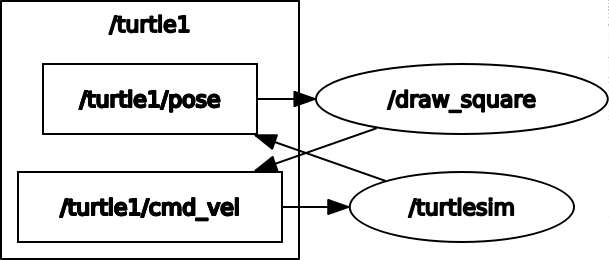
\includegraphics[scale=0.5]{images/turtlesim.png}
    \caption{Grafo della rete turtlesim}
    \label{fig:turtlesim}
\end{figure}
I nodi sono identificati dagli ovali mentre i topic sono identificati dai rettangoli. Vediamo come i due nodi: turtlesim e draw\_square comunicano tra loro tramite i topic \verb+/turtle1/pose+ e \verb+/turtle1/cmd_vel+. Il nodo /draw\_square pubblica sul topic /cmd\_vel la traiettoria per la "tartaruga", questa sarà poi inviata al nodo del simulatore per poi essere eseguita. Quest'ultimo a sua volta pubblicherà la posa del robot al topic /pose che sarà poi letto dal nodo /draw\_square per recuperare la posizione del robot e disegnare la traiettoria.
Il risultato è visibile in figura \ref{fig:turtlesimes}.
\begin{figure}[h!]
    \centering
    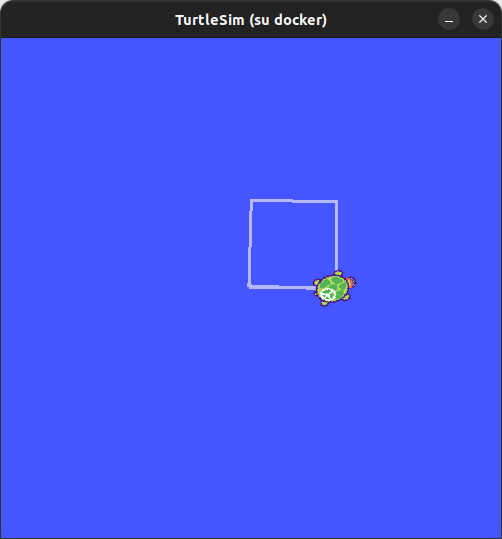
\includegraphics[scale=0.4]{images/turtlesimes.png}
    \caption{Esempio di simulazione turtlesim}
    \label{fig:turtlesimes}
\end{figure}
\section{Architettura utilizzata}
\label{sec:architettura_utilizzata}
In questa sezione mi concentrerò a illustrare l'architettura utilizzata per il mio caso di studio andando anche a definire le milestone indicate nel capitolo \ref{cha:descrizionecasostudio}.
Utilizzerò appunto queste per dare la struttura a questo capitolo, ci erano rimaste da spiegare quindi il wrapping del codice Prolog e la creazione della simulazione.

\subsection{Wrapping codice Prolog}
\label{subsec:wrappping}

\subsection{Simulazione}
\label{subsec:simulation}


      \chapter{Conclusione}
\label{cha:conclusione}
Nel seguente elaborato è stato presentato il mio progetto sia di tirocinio che di tesi triennale. Tutte le fasi dello sviluppo, dalla progettazione alla realizzazione, sono state descritte in modo dettagliato.
In questo capitolo conclusivo verranno presentati i risultati ottenuti e le considerazioni riguardo al progetto sviluppato. Infine verrà dedicata una sezione per le possibili evoluzioni future del progetto.
Iniziamo quindi discutendo dei risultati ottenuti e delle considerazioni.

\section{Risultati ottenuti e considerazioni}
\label{sec:risultati}
Il prodotto finale a cui sono arrivaato è un task planner sviluppato in prolog, il goal principale del planner è quello di risolvere il problema della costruzione di pilastri con dei blocchi di lego.
Questo poi è stato incapsulato in un nodo ROS per rendere il planner utilizzabile in un contesto reale (e simulato). 
Il goal prefissato dal prof. Palopoli, quindi, è stato raggiunto e completato nella sua interezza.

Lo sviluppo di questo progetto mi ha fatto prendere coscienza del mondo della programmazione dichiarativa e della pianificazione automatica. 
Ritengo che Prolog sia uno strumento molto potente che permette di risolvere problemi complessi in modo semplice e veloce.
Prolog è sicuramente uno dei linguaggi che più si adattano a risolvere problemi di questo tipo, le ragioni sono molteplici, qui di seguito elenco quelle che ritengo più importanti:
\begin{itemize}
    \item Paradigma dichiarativo: il programmatore non deve preoccuparsi di come risolvere il problema, ma deve soltanto descriverlo. 
          Questo è particolarmente adatto ai problemi di pianificazione dove è importante descrivere il dominio del problema piuttosto che la soluzione e prolog è perfetto per questo scopo.
    \item Motore di inferenza: Prolog dispone di un motore di inferenza integrato che utilizza un algoritmo di ricerca ad-hoc per raggiungere gli obiettivi specificati dal programma. 
          La potenza sta nell'esplorazione automatica delle soluzioni, questo rende il planner più semplice poichè il ragionamento è delegato al motore di inferenza.
    \item Backtracking: il backtracking consente di esplorare diverse "strade" per raggiungere lo stesso obiettivo. Se una di queste non dovesse funzionare, Prolog "torna indietro" per provarne un'altra fino a trovarne una valida.
    \item Pattern matching: il potente strumento di pattern matching di prolog (unificazione) permette di confrontare stati con obiettivi e condizioni per stabilire che azione compiere.
    \item Logica del prim'ordine: la logica dei predicati di prim'ordine permette a prolog di essere più espressivo e di poter descrivere in modo più semplice e naturale il dominio del problema.
    \item Rappresentazione della conoscenza: prolog permette di rappresentare la conoscenza in modo semplice e naturale, questo è molto importante per la pianificazione automatica poichè è necessario descrivere il dominio del problema.
\end{itemize} 

Inoltre il progetto mi ha permesso di approfondire le mie conoscenze riguardo al mondo della robotica e dell'intelligenza artificiale affermandone anche il mio interesse. In questi mesi di lavoro il prof. Palopoli ha costruito un vero e proprio team composto dal prof. Roveri, il dott. Lamon e il dott. Saccon.
Essendo questo progetto una sfida nuova che non avevo mai affrontato, ho dovuto svolgere molta ricerca e studio per poterlo portare a termine. Loro sono risultati fondamentali per questo scopo siccome erano sempre disponibili al confronto e alla discussione.

I video demo dei risultati ottenuti sono disponibili nella repository del progetto \cite{gitrepo}.
\section{Sviluppi futuri}
\label{sec:sviluppifuturi}
In questa sezione verranno presentati alcuni possibili sviluppi futuri del progetto. Quelli identificati da me sono principalmente 3 ma questo non significa che le possibilità di sviluppo siano limitate a queste. Riporto qui di seguito i possibili sviluppi futuri identificati:
\begin{itemize}
      \item Temporalizzazione delle azioni per una scelta più efficiente del piano da eseguire.
      \item Istanziamento dei fatti tramite rete neurale.
      \item Scenari di paralelizzazione con più agenti (legato molto al primo punto).
\end{itemize}

\subsection*{Temporalizzazione delle azioni}
\label{subsec:temporalizzazione}
In questo progetto le azioni sono sequenziali e atemporali, questo significa che non è possibile eseguire più azioni contemporaneamente e che non è possibile specificare il tempo di esecuzione di un'azione.
Oltre a queste implicazioni la scelta del piano non è ottimizzata quindi non verrà scelto il piano più veloce ma il primo che rispetta i vincoli.

Un lavoro futuro potrebbe essere quindi quello di aggiungere la temporalizzazione delle azioni e i vincoli temporali tra di esse. Così facendo si potrebbe ottimizzare la scelta del piano utilizzando una strategia di minimizzazione del \textit{makespan}\footnote{Tempo che trascorre da inizio a fine piano}.
Si otterrebbe quindi una scelta del piano con criterio e quindi più efficiente e intelligente. 

Un possibile modo per integrare questo aspetto è quello di usare le varie librerie di CLP\footnote{Constraint Logic Programming} presenti in SWI-Prolog. Questa permette di creare dei vincoli tra variabili e di risolverli in modo efficiente.

\subsection*{Utilizzo di una rete neurale per istanziare i fatti}
\label{subsec:neuralnet}
Un altra possibile evoluzione sarebbe legata all'istanziazione dei fatti. Come già presentato nei precedenti capitoli, i fatti \verb+block/13+ al momento sono \textit{grounded}. 
Questo significa che sono sempre veri siccome sono stati definiti a priori. 

Un possibile miglioramento sarebbe quindi di utilizzare un implementazione di prolog neuroprobabilistica, questo renderebbe possibile istanziare i fatti tramite una rete neurale.
L'idea sarebbe quindi di collegare un sensore, ad esempio una telecamera, al mio programma prolog e di utilizzare i dati ricevuti da essa e una rete neurale per istanziare i fatti \verb+block/13+.
Un implementazione di prolog neuroprobabilistica è \textit{DeepProbLog} \cite{MANHAEVE2021103504} ma ne esistono anche altre.

\subsection*{Scenari di paralelizzazione con più agenti}
\label{subsec:parallel}
L'ultimo scenario identificato è quello della possibilità di paralelizzare il piano per la cooperazione multi-agente.
Questo sviluppo è molto legato al primo punto, infatti per poterlo realizzare è necessario che le azioni siano temporali e che quindi sia possibile eseguirle contemporaneamente.
La sfida quindi sarebbe inizialmente di dividere le azioni che ho identificato in sotto azioni e quindi capire quando la possibilità di cooperazione tra agenti è possibile. 
Il dott. Saccon sta già lavorando su questo aspetto e quindi questo potrebbe essere un possibile sviluppo futuro del progetto che sarà applicato realmente nell'immediato futuro.

      
      
    \endgroup


    % bibliografia in formato bibtex
    %
    % aggiunta del capitolo nell'indice
    \addcontentsline{toc}{chapter}{Bibliografia}
    % stile con ordinamento alfabetico in funzione degli autori
    \bibliographystyle{plain}
    \bibliography{biblio}
%%%%%%%%%%%%%%%%%%%%%%%%%%%%%%%%%%%%%%%%%%%%%%%%%%%%%%%%%%%%%%%%%%%%%%%%%%
%%%%%%%%%%%%%%%%%%%%%%%%%%%%%%%%%%%%%%%%%%%%%%%%%%%%%%%%%%%%%%%%%%%%%%%%%%
%% Nota
%%%%%%%%%%%%%%%%%%%%%%%%%%%%%%%%%%%%%%%%%%%%%%%%%%%%%%%%%%%%%%%%%%%%%%%%%%
%% Nella bibliografia devono essere riportati tutte le fonti consultate 
%% per lo svolgimento della tesi. La bibliografia deve essere redatta 
%% in ordine alfabetico sul cognome del primo autore. 
%% 
%% La forma della citazione bibliografica va inserita secondo la fonte utilizzata:
%% 
%% LIBRI
%% Cognome e iniziale del nome autore/autori, la data di edizione, titolo, casa editrice, eventuale numero dell’edizione. 
%% 
%% ARTICOLI DI RIVISTA
%% Cognome e iniziale del nome autore/autori, titolo articolo, titolo rivista, volume, numero, numero di pagine.
%% 
%% ARTICOLI DI CONFERENZA
%% Cognome e iniziale del nome autore/autori (anno), titolo articolo, titolo conferenza, luogo della conferenza (città e paese), date della conferenza, numero di pagine. 
%% 
%% SITOGRAFIA
%% La sitografia contiene un elenco di indirizzi Web consultati e disposti in ordine alfabetico. 
%% E’ necessario:
%%   Copiare la URL (l’indirizzo web) specifica della pagina consultata
%%   Se disponibile, indicare il cognome e nome dell’autore, il titolo ed eventuale sottotitolo del testo
%%   Se disponibile, inserire la data di ultima consultazione della risorsa (gg/mm/aaaa).    
%%%%%%%%%%%%%%%%%%%%%%%%%%%%%%%%%%%%%%%%%%%%%%%%%%%%%%%%%%%%%%%%%%%%%%%%%%
%%%%%%%%%%%%%%%%%%%%%%%%%%%%%%%%%%%%%%%%%%%%%%%%%%%%%%%%%%%%%%%%%%%%%%%%%%
    

    \titleformat{\chapter}
        {\normalfont\Huge\bfseries}{Allegato \thechapter}{1em}{}
    % sezione Allegati - opzionale
\end{document}
